%begin-include
% TODO: remove all contractions and spelling errors

% Outline of this section
% First we should start with a two-page description of the project with:
% - What are cell signaling pathways
% - What types of computational models we have for these pathways and 
% which one do we use
% - What can we do with those networks and how hard is it to get one to 
% work
% - What are the basic tasks to build a pathway
% - What has Lulu done and what are the limitations of her work
% - How do we intend to surmount those limitations


% Subsection Then we should state the main objectives/challenges of our 
% work
% Subsection Then we should give a short description of the work 


% What are cell signaling pathways and how is it important to study them
% - control how cell behaves in different types of environments
% - cancer cells have bad behavior
% - that's one reason to study signaling networks
Cell Signaling pathways are cascades of chemical interactions that 
allow the communication between the cell environment and the 
cell itself. These pathways are also able to regulate many cell 
functions, including DNA replication, cell division and cell death. We
can observe the functioning of signaling pathways as a mechanism that 
can conform the cell behavior with signals that come from the 
environment conditions in which the cell is placed. The studies of cell 
signaling pathways can lead to determining how cells can respond to 
different stimuli; for instance, with the studies of signaling pathways
activated by a chemical species, one could determine how an unhealthy 
cell would respond to a drug containing this species.

% There are computational models for signaling networks
% - Michaelis Menten equations for chemical interactions
% - With a system of ODES we can then simulate the cell behavior
% - However, the huge number of interactions happening in the cell makes
%   it impossible to consider everything.
% - Therefore we must know 
It's possible to construct mathematical models to represent a set of
chemical reactions and consequently a signaling network. One approach on 
the modeling of those interactions is based on the law of mass action. 
This law proposes that the rate of a chemical reaction is proportional 
to the product of reactants concentrations, i.e we can calculate the 
concentration change rate of a species in an interaction by calculating 
the product of reactants concentrations, up to a multiplying constant. 
If we consider the set of interactions of a signaling pathway, we can
then come up with a system of ordinary differential equations (ODEs) 
that can model the dynamics of the concentration of each chemical 
species from the pathway. Generally, these systems are complex and 
cumbersome, if not impossible, to be solved analytically, therefore we 
resort on computational models that apply numerical methods to 
approximate solutions of these systems.

% How do we create these computational models and what should they do?
In this work, we are interested in computational models that can 
reproduce the behavior of signaling networks, comparing experimental 
measures---generally based on Western blot data---to simulated results.
The figure~\ref{fig:signal_pathway_example} shows a set of interactions
as well as parameters of a model of a signaling network. To create these 
computational models, two main tasks need to be accomplished.

\begin{figure}[!ht]
\centering 
    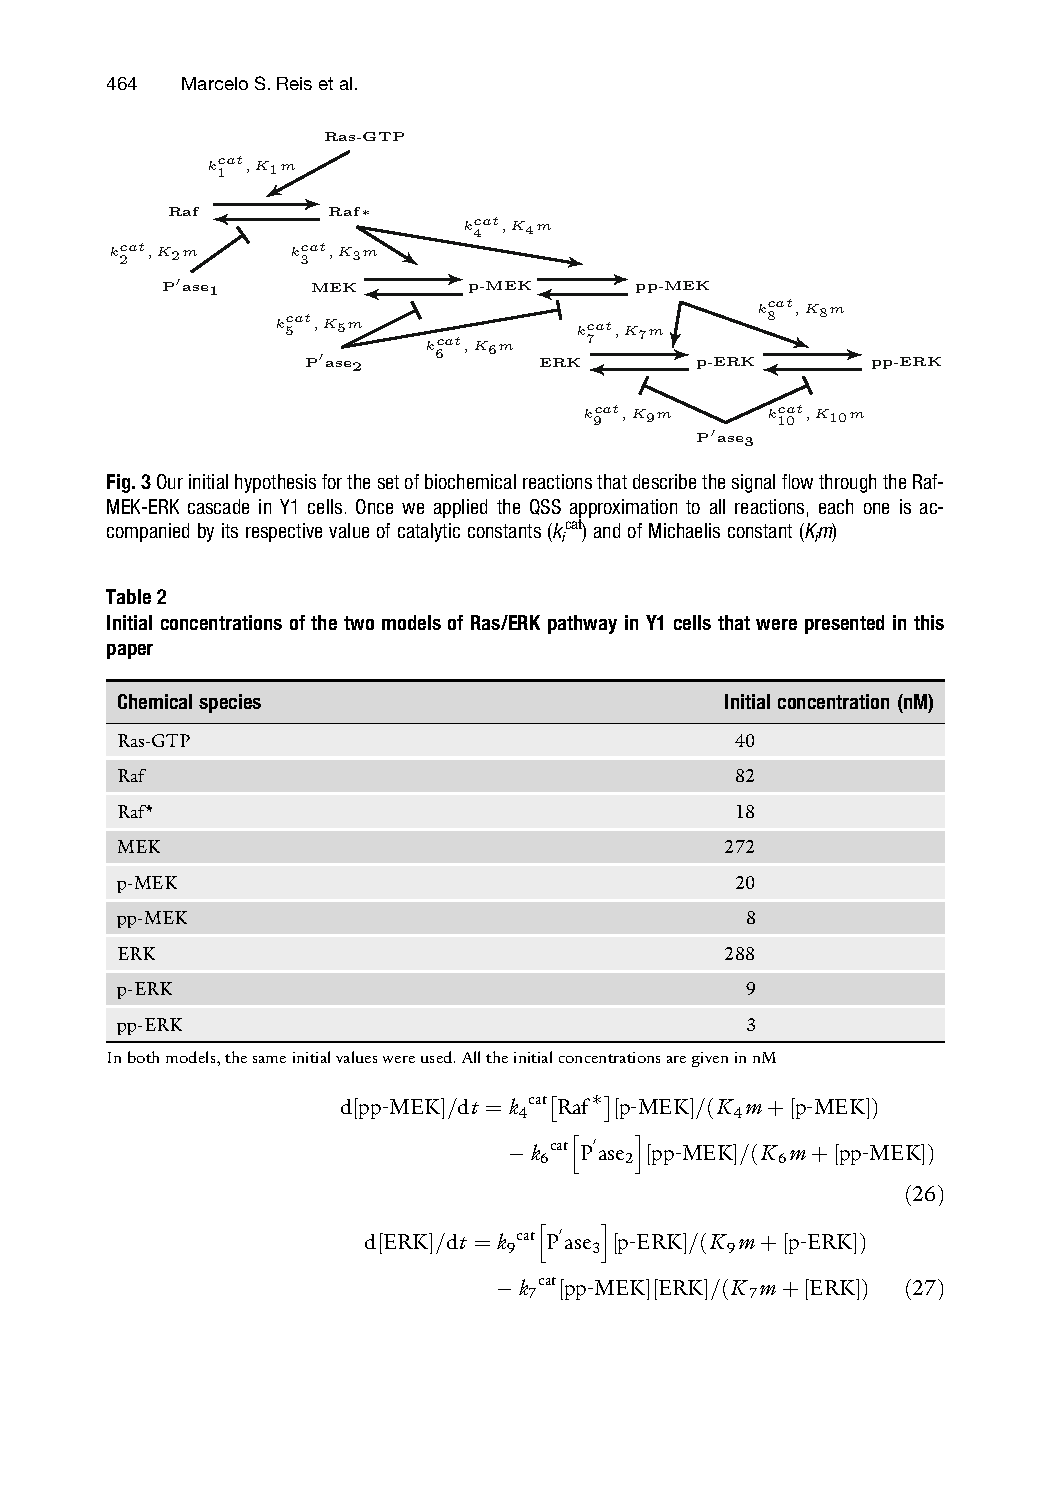
\includegraphics[width=\textwidth, viewport=40 500 460 660, clip]{introduction/signal_pathway_example_full_page.pdf}
\caption{The above diagram show a hypothesis for a signaling pathway 
    that flows through Raf-MEK-ERK cascade. Names in bold represent 
    chemical species. Names in italic represent parameters of the 
    ordinary differential equation of each interaction.Horizontal arrows
    represent phosphorylation when directed from left to right or 
    dephosphorilation when directed in the opposite direction. Other 
    arrows represent positive feedback if they are directed downwards or 
    negative feedback otherwise. Image copied from Marcelo S. Reis et.
    al (2017)~\cite{Reis2017}.}
\label{fig:signal_pathway_example}
\end{figure}

The first task one must complete to create a model is to determine a set 
of interactions to consider in the ODE system. Searching for pathway maps
on the Kyoto Encyclopedia of Genes and Genomes 
(KEGG)~\cite{Kanehisa2000kegg} is a good start. The KEGG PATHWAY 
Database provides manually drawn diagrams that represent signaling 
networks created with experimental evidences. However, it's possible 
that there's no pathway on KEGG that is able to correctly represent the 
biological experiment of interest; for those situations, it's necessary 
to modify the pathway by adding or even removing interactions. One might 
reason that we should use as many interactions as we can to get a better 
simulation, however, this usually implies in poor or computationally 
infeasible models because of two reasons: first, complex models will 
require more time in the numerical solution computation, which may be 
infeasible due to limited computational resources; and second, when 
considering many interactions, we are also placing many parameters 
(multiplying constants of the differential equations) on the model, and 
finding appropriate values for them becomes harder as we increase the 
number of parameters.

The second task to create a model is to find values for all the system
parameters. There are two approaches for this task, you can either 
fetch values for these constants from the literature or you can find 
values that makes the model output approximate the experimental 
observations. For the first approach, repositories such as 
BioModels~\cite{le2006biomodels} can be used; for the second approach, 
statistical and optimization methods can be used. For optimization, it 
is necessary to define a metric that can evaluate how close the 
parameters brings the model output to the experimental observation so
that you can search for the optimal parameter in the parameter space. 
Statistical inference, in the other hand, usually tries to maximize some 
likelihood function, which is defined to represent the probability of a 
model, with a set of parameter values, to reproduce the experimental 
observation.

% However, we might have missed some interactions or even added irrelevant ones
After completing both tasks, however, as we mentioned before, we might 
still not have found a model that fairly approximates the biological 
experiment of interest. That could indicate that the set of chemical 
interactions chosen for the model is incomplete or has interactions that
are not relevant for the biological experiment. Therefore, it is 
desirable to construct a systematic method of modifying the set of 
chemical reactions in order to find the optimal set.

% Lulu solved it as a combinatorial problem
With the title ``A method to modify molecular signaling networks through
examination of interactome databases"~\cite{Wu15} Lulu Wu presented in 
her masters dissertation a methodology to systematically modify 
computational models of signaling networks to better simulate biological 
experiments. Starting with a model that does not approximate well the 
biological data, this methodology proposes to add a set of interactions
to the model topology in order to better simulate the signaling pathway 
of interest. This set of interactions is a subset of interactions from a 
database created by Lulu Wu, joining information
from many static maps available on KEGG. The choice of this subset can 
be modeled as a combinatorial optimization problem in which the search 
space is the set of all possible subsets of interactions to be added.
The cost function of this problem, however, is not as simple to define 
as the search space. Note that the search space itself does not define 
models, but only the topology, i.e. the set of interactions, therefore, 
to consider the second task of creating computational models for 
signaling networks, the cost function must take into account the set of 
values for the model parameters. As an example, we could define the cost 
as the minimum distance between model and experimental measures 
considering all possibilities of parameter values; however, 
unfortunately, finding the minimizing parameter values is a hard 
problem.

Since this is a hard problem, the method presented by Lulu Wu 
implements a heuristic version of this cost function. This heuristics 
is based on a Simulated Annealing procedure that searches for a set of 
parameter values trying to minimize (as much as possible) the distance 
between model and experimental measures; the best found distance is then
considered as the cost of the model. Once the number of possible model 
topologies grows exponentially on the number of interactions from the 
database, the algorithm used to traverse the search space of subset of 
interactions is also a heuristic, and it is based on the greedy 
algorithm called Sequential Forward Selection (SFS)~\cite{Whitney1971}.
The heuristic implemented by Lulu Wu selects a fixed number of 
interactions from the database and then creates candidate models by 
adding to the current solution the respective interaction; then, after 
evaluating the cost function for each model, the algorithm moves to the 
best candidate.

%The work of Lulu Wu was succesful on 

% Her work however had a few flaws...
% To surmount these limitations
% - gather information from many data sources
% - create new search algorithms
% - use Bayesian approach 
